\chapter{Overview}
\label{cha:overview}

This chapter is informal introduction to the RFSM language and of how to use it to describe 
FSM-based systems, simulate them and generate code from these descriptions.

A formal description of the language syntax can be found in Appendix~A.

Future versions of this document will also provide a description of the formal semantics of the
underlying models.

\section{First example}
\label{sec:first-example}

Let's consider the source program given in Listing~\ref{lst:rfsm-example}, whih describes a
simplified mouse controler\footnote{This program is  provided in the distribution, under directory
  \texttt{examples/single/mousectlr}.}. The system is delimited in Fig.~\ref{fig:rfsm-example-delim}. Its
expected behavior is as follows : Input \verb|Top| is supposed to be periodic and hence provide an time base. Whenever an
event occurs on the input \verb|Clic|, an event is emitted either on \verb|DoubleClic| or
\verb|SimpleClic| depending on whether the \verb|Clic| event is followed by another before \verb|D|
events occur on the \verb|Top| input.

\begin{figure}[h]
   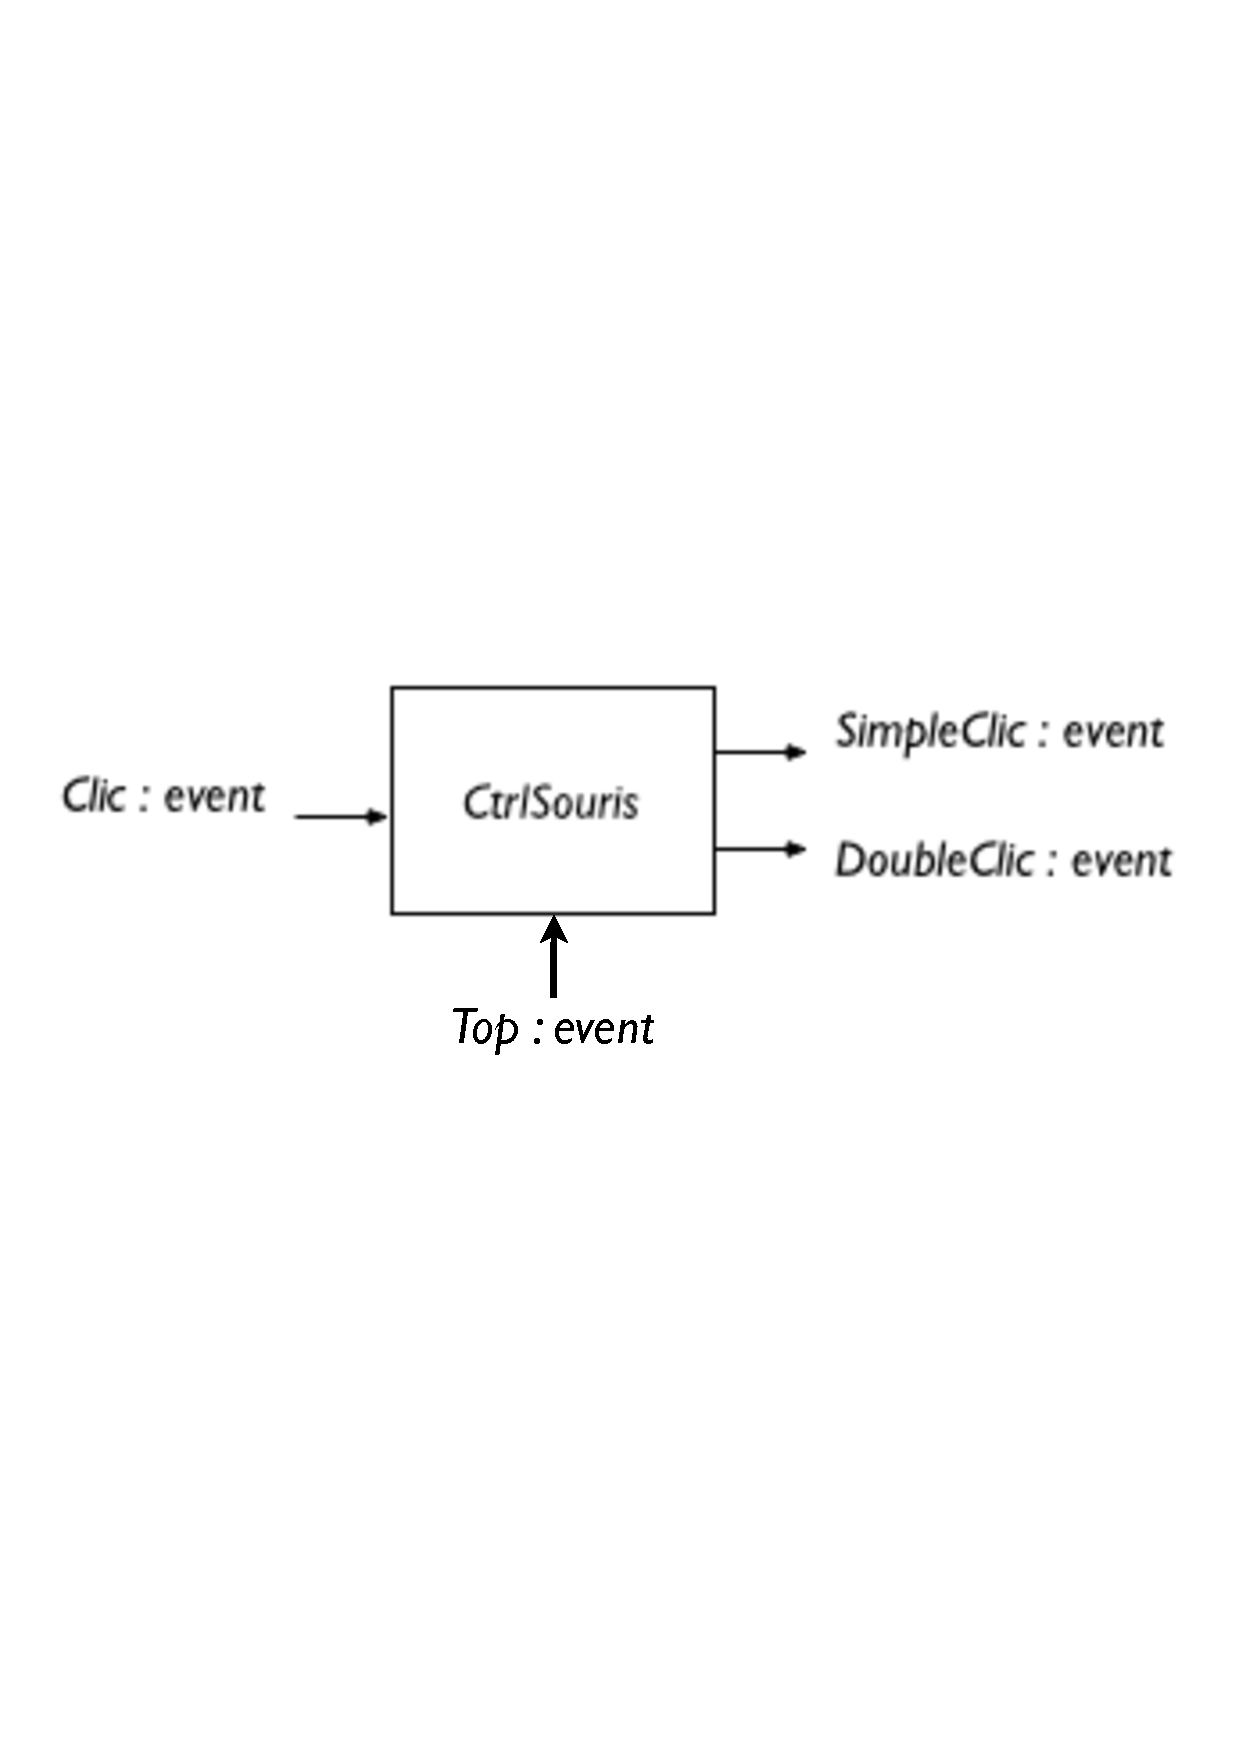
\includegraphics[width=0.5\textwidth]{figs/ctlsouris-delim}
   \centering
  \caption{System delimitation for a (simplified) mouse controler}
  \label{fig:rfsm-example-delim}
\end{figure}


The program itself is composed of three sections :
\begin{itemize}
\item a declaration of an \textbf{FSM model} (lines 1--15),
\item a list of declarations of \textbf{global inputs and outputs} (lines 17--20),
\item an instanciation of the previously declared model (line 22).
\end{itemize}

Let's consider these three sections one after the other.

\begin{lstlisting}[language=Rfsm,frame=single,numbers=left,caption=An RSFM
  program,label={lst:rfsm-example},float]
fsm model ctlr<D:int> (
  in Top: event,
  in Clic: event,
  out SimpleClic: event,
  out DoubleClic: event)
  {
  states:  Idle, Wait;
  vars:  ctr: int<0..D>;
  trans:
    Idle -- Clic | ctr:=0 -> Wait,
    Wait -- Clic | DoubleClic -> Idle,
    Wait -- Top.ctr<D-1 | ctr:=ctr+1 -> Wait,
    Wait -- Top.ctr=D-1 | SimpleClic -> Idle;
  itrans: -> Idle;
  }

input Clk: event = periodic(10,10,120)
input Clic: event = sporadic(25,75,95)
output SClic: event
output DClic: event

fsm c1 = ctlr<5>(Top,Clic,SClic,DClic)
\end{lstlisting}

\subsection*{FSM model}
\label{sec:fsm-model}

An FSM model, introduced by the \verb|fsm model| keyword, describes the interface and behavior of a
\emph{reactive finite state machine}. A reactive finite state machine is a finite state machine
whose transitions can only be caused by the occurrence of \emph{events}.

Here, the declared model, \verb|ctlr|, has two \emph{inputs}, \verb|Top| and
\verb|Clic|, and two \emph{outputs}, \verb|SimpleClic| and \verb|DoubleClic|, all of \verb|event|.
It also has a \emph{parameter}, named \verb|D|, of type \verb|int|. The name of the model, its
inputs, outputs and parameters define its \emph{interface}. 

Following the interface, and between \verb|{ ... }| is the model \emph{body}. This body here
comprises four sections :
\begin{itemize}
\item a section giving a list of possible \emph{states} (line 7),
\item a section introducing a local (internal) \emph{variable} (line 8),
\item a section giving a set of \emph{transition rules} (lines 9--13),
\item a section specifying an \emph{initial transition} (line 14).
\end{itemize}

The behavior of the model itself is entirely specified by the transitions expressed in the
\verb|trans:| and \verb|itrans:| sections.

\medskip
\textbf{Non-initial transitions} are denoted 

\begin{verbatim}
                           src -- cond | acts -> dst
\end{verbatim}

where
\begin{itemize}
\item \texttt{src} is the source state,
\item \texttt{dst} is the destination state,
\item \texttt{cond} is the condition trigerring the transition,
\item \texttt{acts} is a list of actions performed when then transition is enabled.
\end{itemize}

\medskip The semantics is that the transition is enabled whenever the FSM is in the source state and
the triggering condition is true. The associated actions are then performed and the FSM moves to the
destination state.

\medskip
A \textbf{condition} must involve exactly one \emph{triggering event} and, possibly, a conjunction of boolean
conditions called \emph{guards}. The triggering event must be listed in the inputs. The guards may
involve inputs and/or internal variables.

\medskip The \texttt{actions} associated to a transition consists in modifications of the outputs
and/or internal variables or emissions of events.  The set of actions may be empty. In this case,
the transition is denoted :

\begin{verbatim}
                           src -- cond -> dst
\end{verbatim}

\medskip
\textbf{Initial transitions} are denoted 

\begin{verbatim}
                           -> | acts -> dst
\end{verbatim}

where
\begin{itemize}
\item \texttt{dst} is the destination (initial) state,
\item \texttt{acts} is a list of actions associated to this transition (and hence performed at
  initialisation).
\end{itemize}

\medskip
For example, the transitions for the \verb|ctlr| model in Listing.~\ref{lst:rfsm-example}
(lines 10--14) respectively say that
\begin{itemize}
\item the model switches from state \verb|Idle| to state \verb|Wait|, resetting the internal variable
  \verb|ctr| to 0, whenever an event occurs on its \verb|Clic| input;
\item the model switches from state \verb|Wait| to state \verb|Idle|, emitting event
  \verb|DoubleClic|, whenever an event occurs on its \verb|Clic| input;
\item the model stays in state \verb|Wait| but increments the internal variable \verb|ctr| whenever and event occurs
on its \verb|Top| input and that, at this instant, the value of variable \verb|ctr| is less than
\verb|D-1|;
\item the model switches from state \verb|Wait| to state \verb|Idle|, emitting an event on output
\verb|SimpleClic|, whenever and event occurs on its input \verb|Top| and that, at this instant, the
value of variable \verb|ctr| is equal to \verb|D-1|,
\item the model is initially in state \verb|Idle|.
\end{itemize}

A graphical representation of the corresponding FSM is given in
Fig.~\ref{fig:rfsm-example-dot}.  This representation was actually automatically generated from the
program (as explained in Chap.~\ref{cha:rfsmc}). 

\begin{figure}[h]
   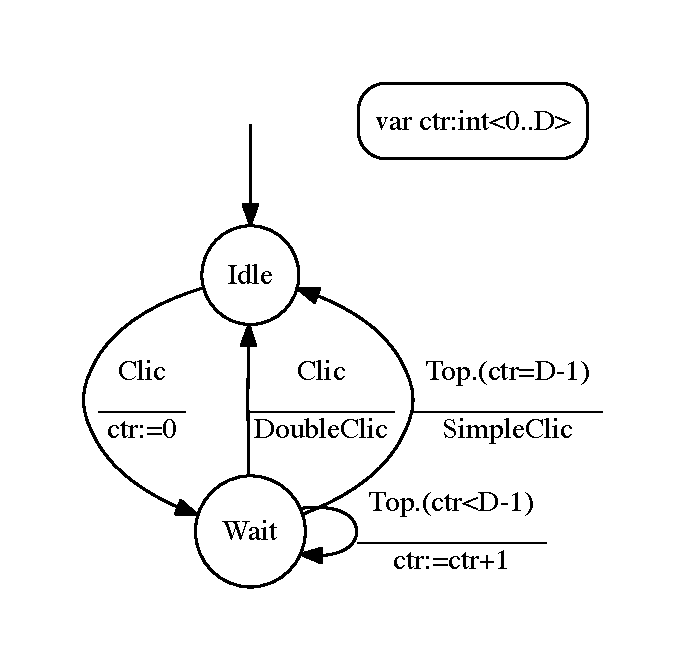
\includegraphics[height=8cm]{figs/ctlsouris-model}
   \centering
  \caption{A graphical representation of the FSM model described in Listing~\ref{lst:rfsm-example}}
  \label{fig:rfsm-example-dot}
\end{figure}

\medskip
Note that, at this level, the value of the parameter \verb|D| used in the guard associated to the
third and fourth transition, is left unspecified, thus providing some kind of \emph{genericity}. 

\subsection*{Globals}
\label{sec:globals}

There are three types of global values : inputs, outputs and shared objects. This section only deals
with global inputs (shared objects will be introduced in Sec.\ref{sec:second-example}). Global inputs  and
outputs represent the interface of the system to the external world. 

\medskip
For global outputs the declaration simply gives a name and a type, as illustrated in lines 19--20 of
Listing~\ref{lst:rfsm-example}. 

\medskip
For global inputs, the declaration also specifies the \textbf{stimuli} which are attached to the
corresponding input for simulating the system. There are three types of stimuli : periodic and
sporadic stimuli for inputs of type \verb|event| and value changes for scalar inputs.
Periodic stimuli are specified with a period, a starting time and an ending time. Sporadic stimuli
are simply a list of dates at which the corresponding input event occurs. Value changes are given as
list of pairs \verb|t:v|, where \verb|t| is a date and \verb|v| the value assigned to the
corresponding input at this date. 

\medskip
For example, in Listing~\ref{lst:rfsm-example}
\begin{itemize}
\item line 17 declares \verb|Clk| as a global input producing periodic events with period 10, starting
  at t=10 and ending at t=100\footnote{Note that, at this level, there's no need for an absolute
    unit for time.},
\item line 18 declares \verb|Clic| as a global input producing events at t=25, t=75 and
  t=95.
\end{itemize}

\medskip
A program making use, for example, of a boolean input \verb|Enable| initially at 0, then going to 1 at t=25 and
back to 0 at t=35 would declare :

\begin{lstlisting}[language=Rfsm,frame=single]
input Enable : bool = value_changes (0:0, 25:1, 35:0)
\end{lstlisting}

\subsection*{FSM instances}
\label{sec:fsm-instances}

The last section of an RFSM program constructs the description of the system by instanciating
-- and, possibly, inter-connecting -- the previously FSM models.
Instanciating a model creates a ``copy'' of the corresponding FSM for which
\begin{itemize}
\item the value of the declared generic parameter,
\item the declared inputs and outputs are actually connected to global inputs, outputs or shared
  objects.
\end{itemize}

In the program of Listing~\ref{lst:rfsm-example}, instanciation of the \verb|ctlr| model takes place
at line 22 and creates an instance named \verb|c1|, for which
\begin{itemize}
\item the parameter \verb|D| has value 5,
\item the inputs \verb|Top| and \verb|Clic| (resp. outputs \verb|SimpleClic|, \verb|DoubleClic|) are bound to
  the global inputs \verb|Top| and \verb|Clk|  (resp. outputs  \verb|SClic| and \verb|DClic|).
\end{itemize}

\subsection*{Drawing}
\label{sec:drawing-1}

As stated above, it is straightforward to obtain -- either using the commmand-line compiler
described in chapter~\ref{cha:rfsmc} or the IDE described in chapter~\ref{cha:gui} -- a graphical
representation the program in Listing~\ref{lst:rfsm-example}. The corresponding diagram is here
reproduced in Fig.~\ref{fig:rfsm-example-top}.

\begin{figure}[h]
   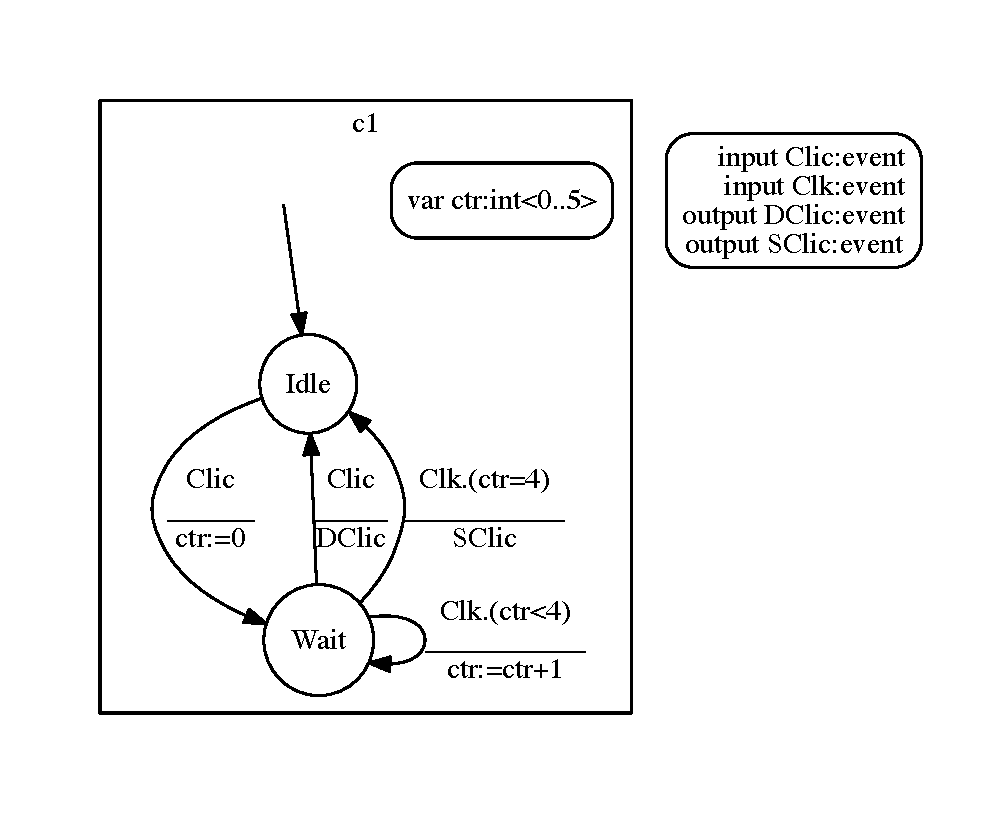
\includegraphics[height=9cm]{figs/ctlsouris-top}
   \centering
  \caption{A graphical representation of program described in Listing~\ref{lst:rfsm-example}}
  \label{fig:rfsm-example-top}
\end{figure}

% \medskip
% A legitimate question is whether RFSM has chosen to \emph{derive} graphical models from textual ones
% instead of specifying systems graphically right from the start (using some kind of graphical FSM
% editor, as provided by some existing tools).

% The reason is that purely graphical specifications, although appealing at first sight, indeed have
% several limitations. TBC...
  
\subsection*{Simulating}
\label{sec:simulating-1}

Simulating the program means computing the reaction of the FSM instances to the input stimuli. This
is also straightforward using the RFSM command-line compiler or IDE. Simulation produces a set of
\emph{traces} in VCD (Value Change Dump) format which can visualized using \emph{waveform viewers}
such as \texttt{gtkwave}. The simulation results for the program in Listing~\ref{lst:rfsm-example}
are illustrated in Fig.~\ref{fig:rfsm-example-vcd}.

\begin{figure}[h]
   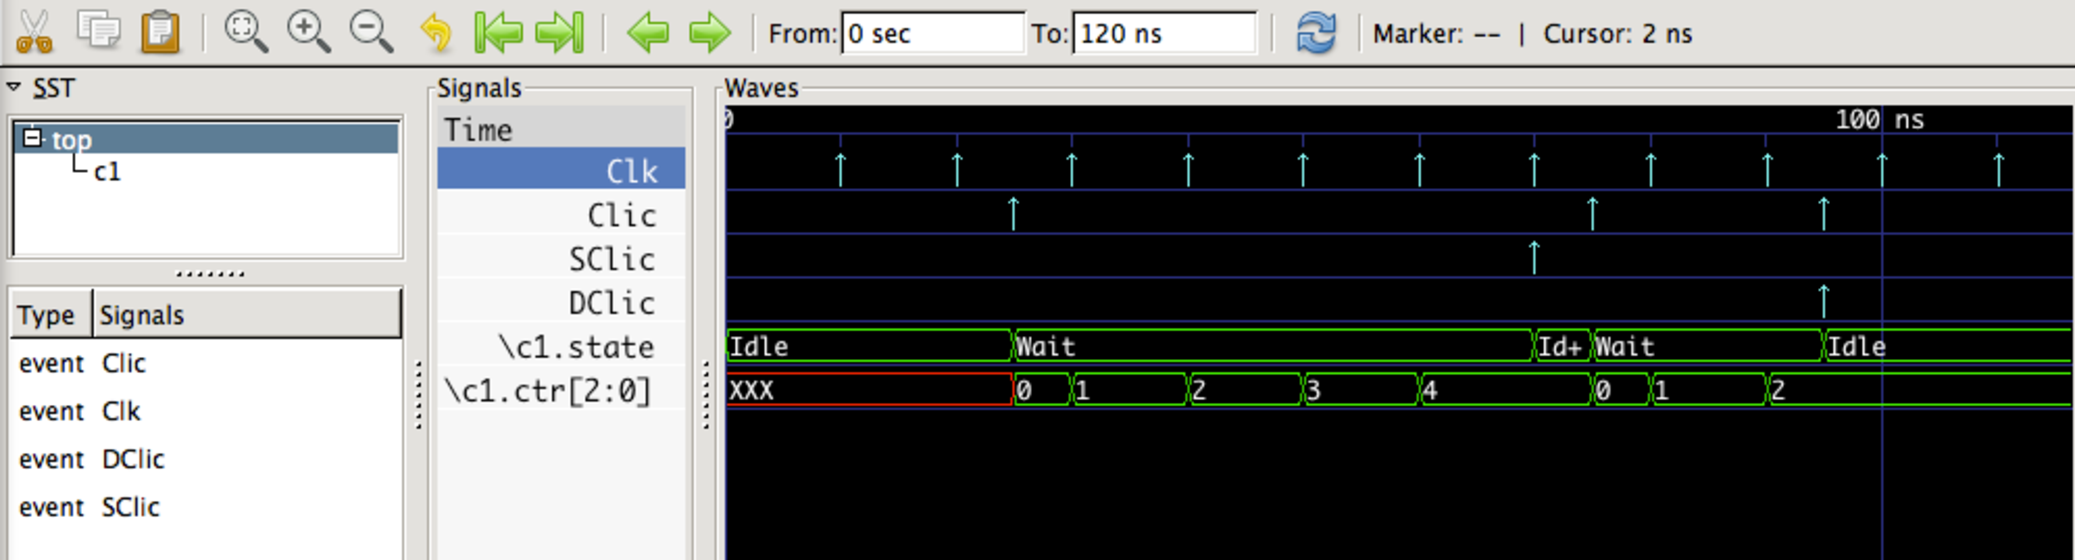
\includegraphics[width=\textwidth]{figs/ctlsouris-chrono}
   \centering
  \caption{Simulation results for the program in Listing~\ref{lst:rfsm-example}, viewed using
    \texttt{gtkwave}}
  \label{fig:rfsm-example-vcd}
\end{figure}

\subsection*{Code generation}
\label{sec:code-generation-1}

RFSM can also generate code implementing the FSM models and their environment for simulation and/or
integration to existing applications.

\medskip
Currently, three backends are provided :
\begin{itemize}
\item a backend generating a C-based implementation of each FSM instance,
\item a backend generating a \emph{testbench} implementation in SystemC (FSM instances + stimuli
  generators),
\item a backend generating a \emph{testbench} implementation in VHDL (FSM instances + stimuli
  generators).
\end{itemize}

\medskip
The target language for the C backend is a C-like language augmented with
\begin{itemize}
\item a \verb|task| keyword for naming generated behaviors,
\item \verb|in| and \verb|out| keywords for identifying inputs and outputs,
\item a builtin \verb|event| type,
\item primitives for handling events : \verb|wait_ev()|, \verb|verb|wait_evs()| and
  \verb|notify_ev()|. 
\end{itemize}
The idea is that the generated code can be turned into an application for a multi-tasking operating
system by providing actual implementations of the corresponding constructs and primitives.

\medskip
For the SystemC and VHDL backends, the generated code can actually be compiled and executed for
simulation purpose and. The FSM implementations generated by the VHDL backend can also be
synthetized to be implemented hardware using hardware-specific tools\footnote{We use the
  \textsc{quartus} toolchain from Intel/Altera.}. 

\medskip
Appendices C1 and C2 respectively give the C and SystemC code generated from the example in
Listing~\ref{lst:rfsm-example}. 

\medskip
\textbf{Note}. The current VHDL backend does not support multi-FSM models, nor FSM models having
more than one input event. These limitations may be removed in future versions.

\section{Second exemple}
\label{sec:second-example}

This second example is only for illustrating the generation of VHDL code.  The program is given in
Listing~\ref{lst:rfsm-example2}. The modelized system is a calibrated pulse generator\footnote{This
  program is provided in the distribution, under directory
  \texttt{examples/single/gensig/v2}.}. Given an input clock \verb|H|, with period $T_H$, it
generates a pulse of duration $n \times T_H$ whenever input \texttt{E} is set when event $H$
occurs. The generic model \verb|gensig| is here instanciated with \verb|N=4|.

\begin{lstlisting}[language=Rfsm,frame=single,numbers=left,caption=A multi-model RFSM
  program,label={lst:rfsm-example2},float]

fsm model gensig<n:int> (
  in h: event,
  in  e: bool,
  out s: bool)
  {
  states: E0, E1;
  vars: k: int<0..n>;
  trans: 
    E0 -- h.e=1 | k:=1; s:=1 -> E1,
    E1 -- h.k<n | k:=k+1 -> E1,
    E1 -- h.k=n | s:=0 -> E0;
  itrans: | s:=0 -> E0;
  }

input H : event = periodic (10,0,80)
input E : bool = value_changes (0:0, 25:1, 35:0)
output S : bool 

fsm g4 = gensig<4>(H,E,S)
\end{lstlisting}

\medskip
The graphical representation of the program is given in Fig.~\ref{fig:rfsm-example2-top}. Simulation
results are illustrated in Fig~\pageref{fig:rfsm-example2-vcd}. 
Appendix C3 gives the VHDL code generated from this example.

\begin{figure}[h]
   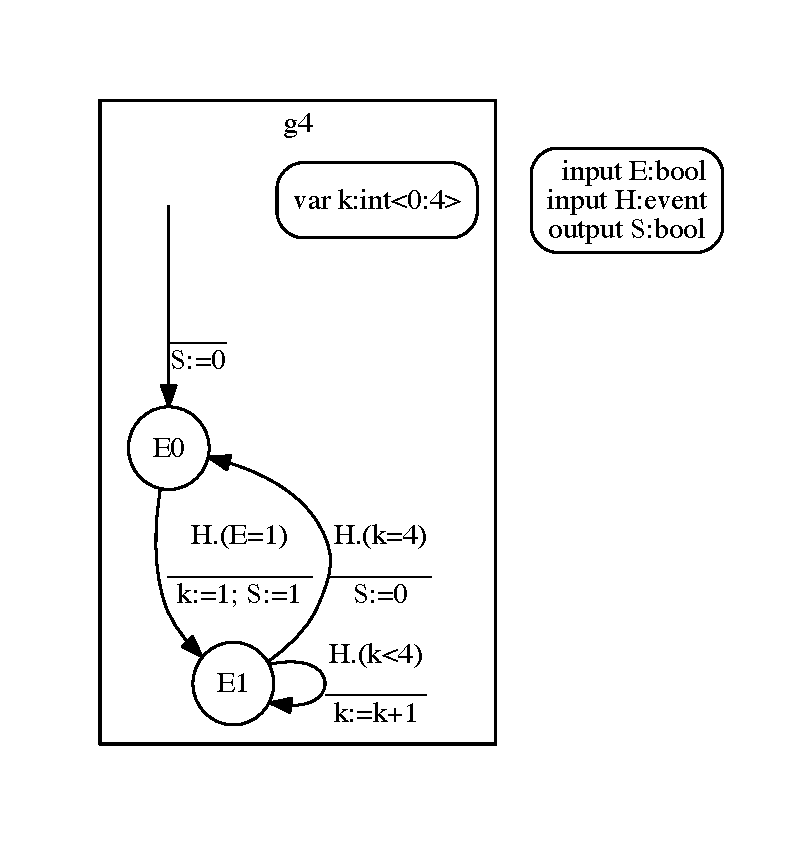
\includegraphics[height=9cm]{figs/gensig-top}
   \centering
  \caption{A graphical representation of program described in Listing~\ref{lst:rfsm-example2}}
  \label{fig:rfsm-example2-top}
\end{figure}

\begin{figure}[h]
   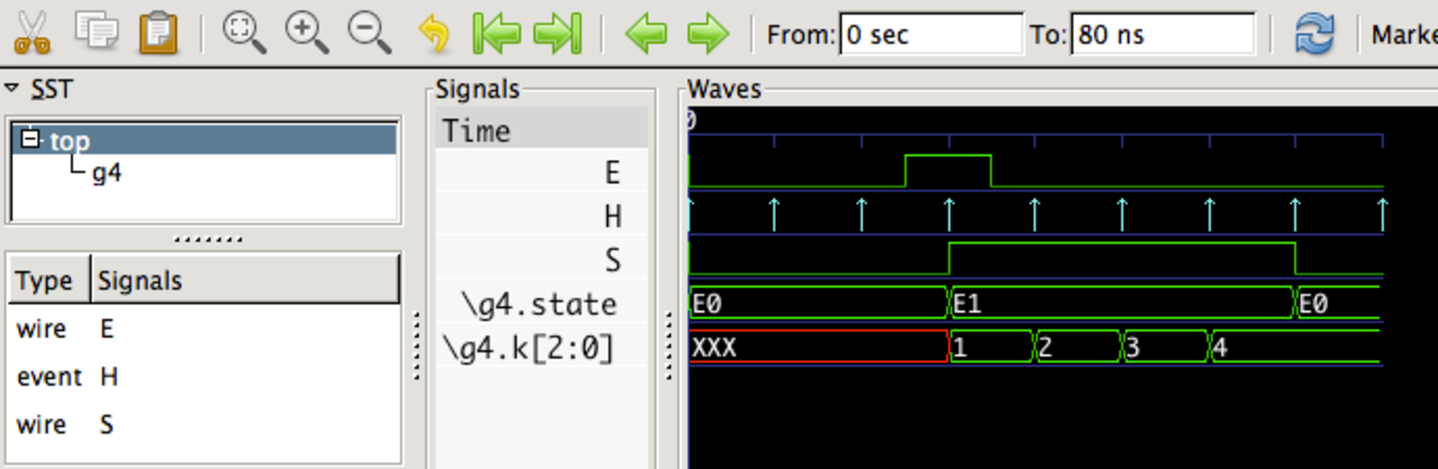
\includegraphics[width=\textwidth]{figs/gensig-chrono}
   \centering
  \caption{Simulation results for the program in Listing~\ref{lst:rfsm-example2}}
  \label{fig:rfsm-example2-vcd}
\end{figure}

\section{Third exemple}
\label{sec:third-exemple}

In this third example, we consider a multi-FSM model. The program is given in
Listing~\ref{lst:rfsm-example3}. The system is a simple modulo 8 counter, here described as a
combination of three event-synchronized modulo 2 counters\footnote{This program is provided in the
  distribution, under directory \texttt{examples/multi/ctrmod8}.}.

\medskip
Here a single FSM model (\texttt{cntmod2}) is instanciated thrice, as \texttt{C0}, \texttt{C1} and
\texttt{C2}. These instances are synchronized using two \textbf{shared events}, \texttt{R0} and \texttt{R1}. 

\medskip
The graphical representation of the program is given in Fig.~\ref{fig:rfsm-example3-top}. Simulation
results are illustrated in Fig~\pageref{fig:rfsm-example3-vcd}. 

\begin{lstlisting}[language=Rfsm,frame=single,numbers=left,caption=A multi-model RFSM
  program,label={lst:rfsm-example3},float]
fsm model cntmod2 (
  in h: event,
  out s: int<0..1>,
  out r: event)
  {
  states: E0, E1;
  trans:
    E0 -- h | s:=1 -> E1,
    E1 -- h | r; s:=0 -> E0;
  itrans: | s:=0 -> E0;
  }

input H: event = periodic(10,10,100)
output S0: int<0..1>
output S1: int<0..1>
output S2: int<0..1>
output R2: event

shared R0: event
shared R1: event

fsm C0 = cntmod2(H,S0,R0) 
fsm C1 = cntmod2(R0,S1,R1) 
fsm C2 = cntmod2(R1,S2,R2) 
\end{lstlisting}

\begin{figure}[h]
   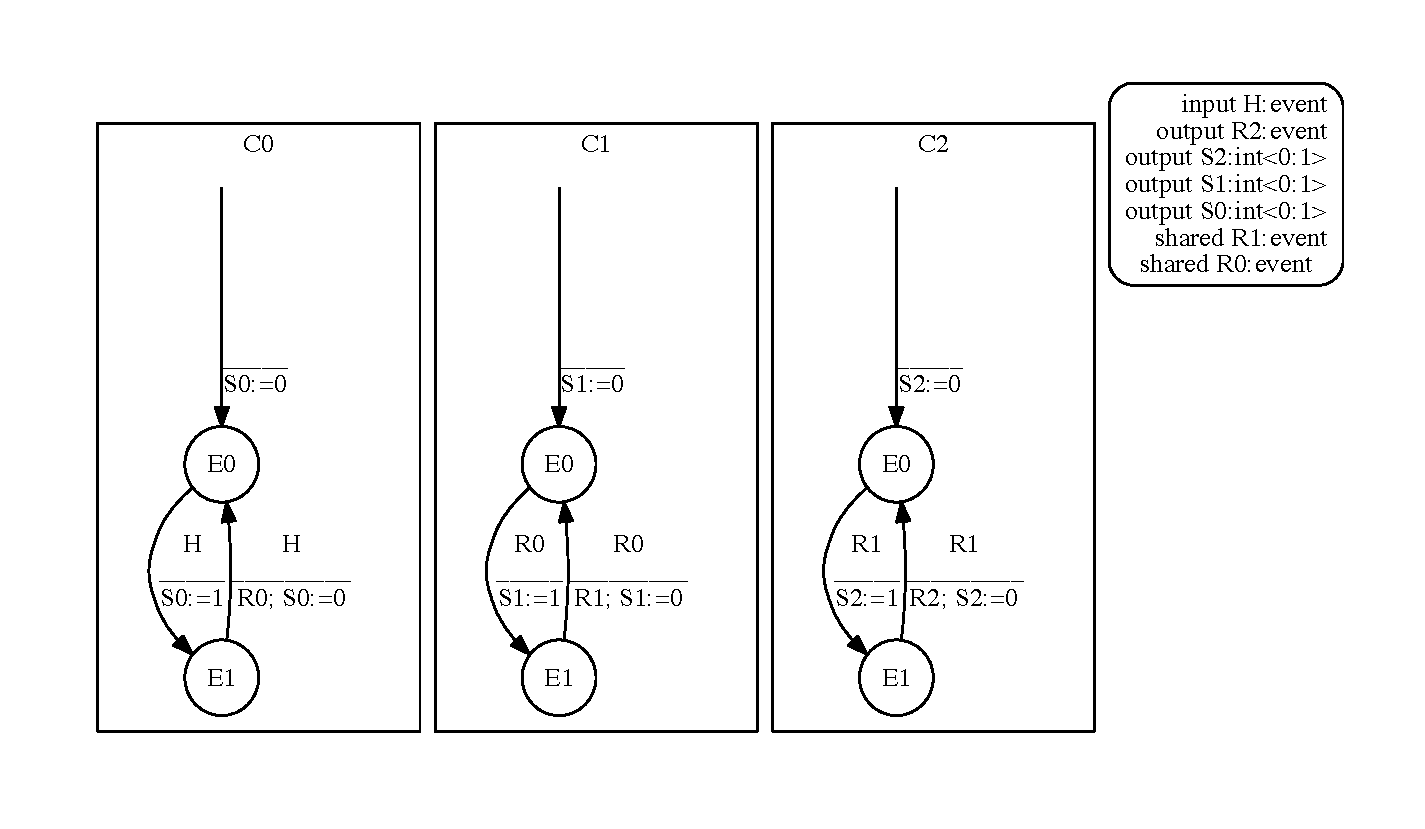
\includegraphics[height=9cm]{figs/ctrmod8-top}
   \centering
  \caption{A graphical representation of program described in Listing~\ref{lst:rfsm-example3}}
  \label{fig:rfsm-example3-top}
\end{figure}

\begin{figure}[h]
   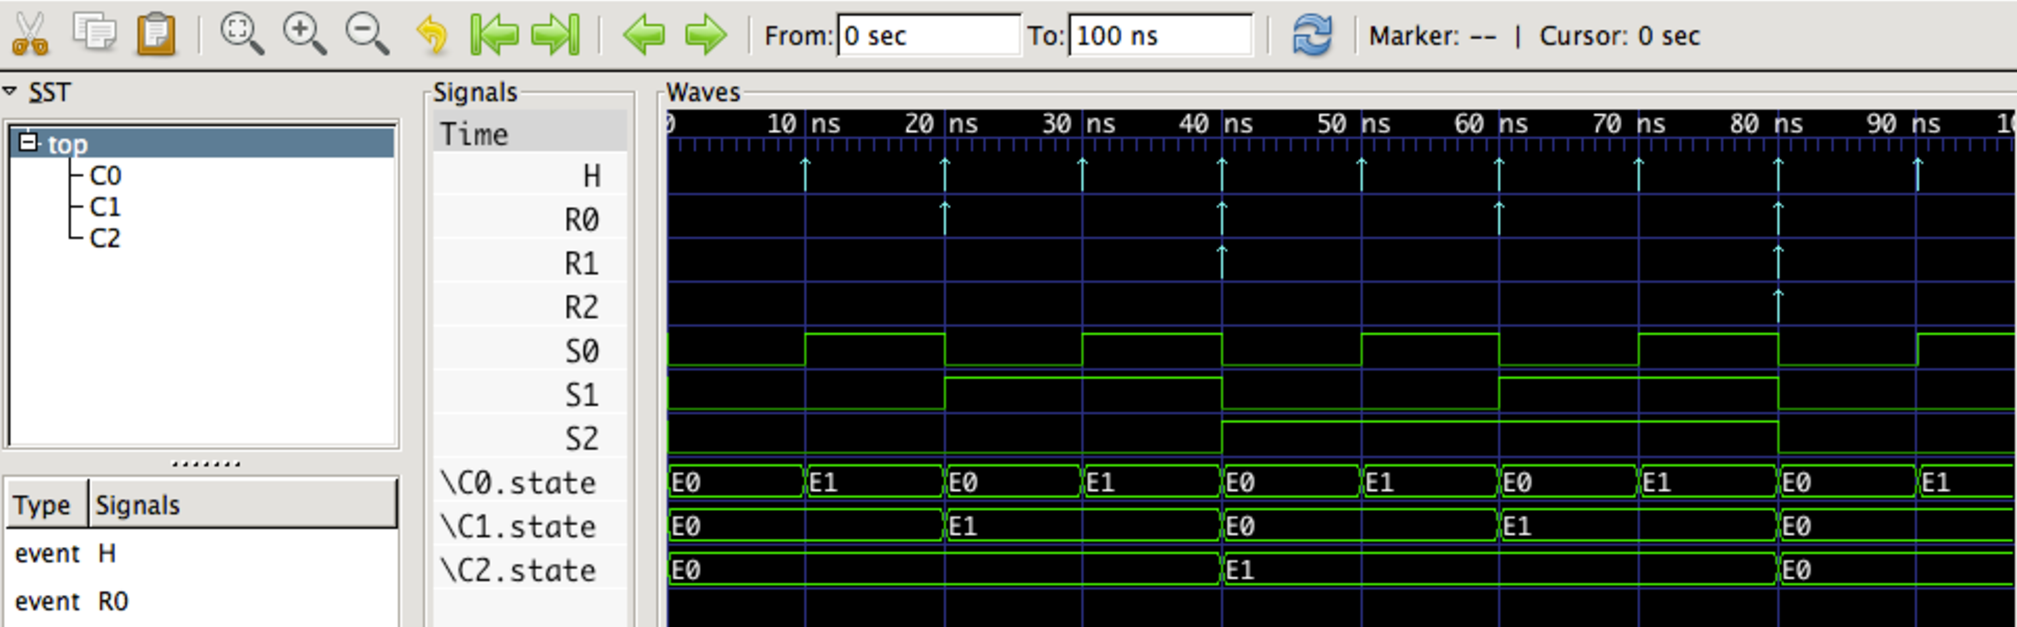
\includegraphics[width=\textwidth]{figs/ctrmod8-chrono}
   \centering
  \caption{Simulation results for the program in Listing~\ref{lst:rfsm-example3}}
  \label{fig:rfsm-example3-vcd}
\end{figure}

%%% Local Variables: 
%%% mode: latex
%%% TeX-master: "rfsm"
%%% End: 
